%%%%%%%%%%%%%%%%%%%%%%%%%%%%%%%%%%%%%%%%%%%%%%%%%%%%%%%%
\documentclass[12pt,a4paper]{article}% 文档格式
\usepackage{ctex,hyperref}% 输出汉字
\usepackage{times}% 英文使用Times New Roman
%%%%%%%%%%%%%%%%%%%%%%%%%%%%%%%%%%%%%%%%%%%%%%%%%%%%%%%%
\title{\fontsize{18pt}{27pt}\selectfont% 小四字号,1.5倍行距
	{\heiti% 黑体 
	物联网:一项调查}}% 题目
%%%%%%%%%%%%%%%%%%%%%%%%%%%%%%%%%%%%%%%%%%%%%%%%%%%%%%%%
\author{\fontsize{12pt}{18pt}\selectfont% 小四字号,1.5倍行距
	{\fangsong% 仿宋
	Luigi Atzori, Antonio Iera, Giacomo Morabito}\\% 标题栏脚注
	}% 作者单位,“~”表示空格
%%%%%%%%%%%%%%%%%%%%%%%%%%%%%%%%%%%%%%%%%%%%%%%%%%%%%%%%
\date{}% 日期(这里避免生成日期)
%%%%%%%%%%%%%%%%%%%%%%%%%%%%%%%%%%%%%%%%%%%%%%%%%%%%%%%%
\usepackage{amsmath,amsfonts,amssymb}% 为公式输入创造条件的宏包
%%%%%%%%%%%%%%%%%%%%%%%%%%%%%%%%%%%%%%%%%%%%%%%%%%%%%%%%
\usepackage{graphicx}% 图片插入宏包
\usepackage{subfigure}% 并排子图
\usepackage{float}% 浮动环境,用于调整图片位置
\usepackage[export]{adjustbox}% 防止过宽的图片
%%%%%%%%%%%%%%%%%%%%%%%%%%%%%%%%%%%%%%%%%%%%%%%%%%%%%%%%
\usepackage{bibentry}
\usepackage{natbib}% 以上2个为参考文献宏包
%%%%%%%%%%%%%%%%%%%%%%%%%%%%%%%%%%%%%%%%%%%%%%%%%%%%%%%%
\usepackage{abstract}% 两栏文档,一栏摘要及关键字宏包
\renewcommand{\abstracttextfont}{\fangsong}% 摘要内容字体为仿宋
\renewcommand{\abstractname}{\textbf{摘\quad 要}}% 更改摘要二字的样式
%%%%%%%%%%%%%%%%%%%%%%%%%%%%%%%%%%%%%%%%%%%%%%%%%%%%%%%%
\usepackage{xcolor}% 字体颜色宏包
\newcommand{\red}[1]{\textcolor[rgb]{1.00,0.00,0.00}{#1}}
\newcommand{\blue}[1]{\textcolor[rgb]{0.00,0.00,1.00}{#1}}
\newcommand{\green}[1]{\textcolor[rgb]{0.00,1.00,0.00}{#1}}
\newcommand{\darkblue}[1]
{\textcolor[rgb]{0.00,0.00,0.50}{#1}}
\newcommand{\darkgreen}[1]
{\textcolor[rgb]{0.00,0.37,0.00}{#1}}
\newcommand{\darkred}[1]{\textcolor[rgb]{0.60,0.00,0.00}{#1}}
\newcommand{\brown}[1]{\textcolor[rgb]{0.50,0.30,0.00}{#1}}
\newcommand{\purple}[1]{\textcolor[rgb]{0.50,0.00,0.50}{#1}}% 为使用方便而编辑的新指令
%%%%%%%%%%%%%%%%%%%%%%%%%%%%%%%%%%%%%%%%%%%%%%%%%%%%%%%%
\usepackage{url}% 超链接
\usepackage{bm}% 加粗部分公式
\usepackage{multirow}
\usepackage{booktabs}
\usepackage{epstopdf}
\usepackage{epsfig}
\usepackage{longtable}% 长表格
\usepackage{supertabular}% 跨页表格
\usepackage{algorithm}
\usepackage{algorithmic}
\usepackage{changepage}% 换页
%%%%%%%%%%%%%%%%%%%%%%%%%%%%%%%%%%%%%%%%%%%%%%%%%%%%%%%%
\usepackage{enumerate}% 短编号
\usepackage{caption}% 设置标题
\captionsetup[figure]{name=\fontsize{10pt}{15pt}\selectfont Figure}% 设置图片编号头
\captionsetup[table]{name=\fontsize{10pt}{15pt}\selectfont Table}% 设置表格编号头
%%%%%%%%%%%%%%%%%%%%%%%%%%%%%%%%%%%%%%%%%%%%%%%%%%%%%%%%
\usepackage{indentfirst}% 中文首行缩进
\usepackage[left=2.50cm,right=2.50cm,top=2.80cm,bottom=2.50cm]{geometry}% 页边距设置
\renewcommand{\baselinestretch}{1.5}% 定义行间距(1.5)
%%%%%%%%%%%%%%%%%%%%%%%%%%%%%%%%%%%%%%%%%%%%%%%%%%%%%%%%
\usepackage{fancyhdr} %设置全文页眉、页脚的格式
\pagestyle{fancy}
\hypersetup{colorlinks=true,linkcolor=black}% 去除引用红框,改变颜色
%%%%%%%%%%%%%%%%%%%%%%%%%%%%%%%%%%%%%%%%%%%%%%%%%%%%%%%%

\begin{document}% 以下为正文内容
	\maketitle% 产生标题,没有它无法显示标题
	%%%%%%%%%%%%%%%%%%%%%%%%%%%%%%%%%%%%%%%%%%%%%%%%%%%%%%%%
	\lhead{}% 页眉左边设为空
	\chead{}% 页眉中间设为空
	\rhead{}% 页眉右边设为空
	\lfoot{}% 页脚左边设为空
	\cfoot{\thepage}% 页脚中间显示页码
	\rfoot{}% 页脚右边设为空
	%%%%%%%%%%%%%%%%%%%%%%%%%%%%%%%%%%%%%%%%%%%%%%%%%%%%%%%%
	\begin{abstract}
		\fangsong 本文涉及物联网。这种有希望的模式的主要促成因素是多种技术和通信解决方案的集成。识别和跟踪技术、有线和无线传感器和执行器网络、增强型通信协议(与下一代互联网共享)以及智能物体的分布式智能是最相关的。可以很容易地想象,对物联网发展的任何重大贡献都必然是在电信、信息学、电子和社会科学等不同知识领域进行协同活动的结果。在这样一个复杂的场景中,这项调查针对的是那些希望接触这一复杂学科并为其发展做出贡献的人。报道了这种物联网模式的不同愿景,并回顾了使能技术。现在出现的情况是,研究界仍将面临一些重大问题。其中最相关的部分将详细说明。
	\end{abstract}
	
	\begin{adjustwidth}{1.06cm}{1.06cm}
		\fontsize{10.5pt}{15.75pt}\selectfont{\heiti{关键词:}\fangsong{物联网,普适计算,射频识别系统}}\\
	\end{adjustwidth}
	

	\newpage% 从新的一页继续


\section{介绍}
物联网(IoT)是一种新颖的范式,在现代无线通信场景中正在迅速取得进展。这一概念的基本思想是我们周围无处不在的各种事物或物体——如射频识别(RFID)标签、传感器、执行器、移动电话等——它们通过独特的寻址方案,能够相互交互,并与它们的邻居合作,以达到共同的目标。

毫无疑问,物联网理念的主要优势在于它将对潜在用户日常生活和行为的几个方面产生巨大影响。从私人用户的角度来看,物联网引入的最明显的影响将在工作和家庭领域都可见。
在这种情况下,智能家居技术、辅助生活、电子健康、增强学习只是几个可能的应用场景的例子,在这些场景中,新范式将在不久的将来发挥主导作用。同样,从业务用户的角度来看,最明显的后果将在自动化和工业制造、物流、业务/流程管理、人员和货物的智能运输等领域同样可见。

从上述考虑出发,物联网被美国国家情报委员会列入对美国国力有潜在影响的六项“破坏性民用技术”名单,这并不奇怪。
NIC预计,“到2025年,互联网节点可能存在于日常用品中——食品包装、家具、纸质文件等”。它强调了未来将出现的机遇,从“巨大的需求与技术进步相结合,可以推动物联网的广泛传播,物联网可以像现在的互联网一样,为经济发展做出巨大贡献”的想法开始。还强调了广泛采用这种技术可能带来的威胁。事实上,有人强调,“在日常物品成为信息安全风险的程度上,物联网可以比迄今为止的互联网更广泛地分布这些风险”。

事实上,许多具有挑战性的问题仍需解决,在物联网理念被广泛接受之前,必须解开技术和社会的结。

核心问题是使互连设备的完全互操作性成为可能,通过实现它们的自适应和自主行为,为它们提供始终更高程度的智能,同时保证信任、隐私和安全。此外,物联网的理念也带来了一些关于网络方面的新问题。事实上,构成物联网的东西在计算和能源容量方面都将以低资源为特征。因此,除了明显的可扩展性问题外,所提出的解决方案还需要特别关注资源效率。

一些工业、标准化和研究机构目前正在参与解决方案的开发活动,以满足突出的技术要求。这项调查展示了物联网的现状。更具体地说,它:

1、为读者提供了来自不同科学界的物联网范式的不同愿景的描述;

2、回顾了使能技术,并说明了这种范式在日常生活中传播的主要好处;

3、对科学界仍需面对的主要研究问题进行了分析。

主要目的是让读者有机会了解已经做了什么(协议、算法、提出的解决方案),还有什么需要解决,以及这一进化过程的促成因素是什么,它的弱点和风险因素是什么。

本文的其余部分组织如下。在第2节中,我们介绍并比较了物联网范式的不同愿景,这些愿景可从文献中获得。物联网的主要赋能技术是第3节的主题,而未来将受益于物联网理念的全面部署的主要应用程序的描述在第4节中进行了阐述。第5节通过强调寻址、网络、安全、隐私和标准化工作等主题,简要介绍了研究应更多关注的未决问题。
第6节给出了结论和未来的研究提示。

\section{一种范式,多种愿景}
物联网的多种定义可以在研究界找到,这证明了人们对物联网问题的浓厚兴趣,以及关于物联网的辩论的活跃程度。通过浏览文献,感兴趣的读者可能很难理解物联网的真正含义,这个概念背后的基本思想,以及物联网的全面部署将产生哪些社会、经济和技术影响。

今天围绕这个术语的明显模糊的原因是“物联网”这个名称本身的结果,它在语法上由两个术语组成。第一个是推动物联网面向网络的愿景,而第二个是将重点放在通用“对象”上,将其集成到一个通用框架中。

物联网愿景中的差异,有时是实质性的,是因为利益相关者、商业联盟、研究和标准化机构开始从“以互联网为导向”或“以价值观为导向”的角度来处理这个问题,这取决于他们的具体兴趣、最终结果和背景。

无论如何,我们不应忘记,“互联网”和“互联网”这两个词放在一起,其含义是将颠覆性的创新水平引入当今的信息通信技术世界。事实上,“物联网”在语义上意味着“基于标准通信协议,可唯一寻址的互连对象的全球网络”。这意味着过程中涉及大量(异构)对象。
对象的唯一寻址以及交换信息的表示和存储成为最具挑战性的问题,直接带来了物联网的第三个“面向语义”的视角。

在图1中,重点介绍了主要概念、技术和标准,并根据它们有助于最佳表征的物联网愿景进行了分类。从这样的例子来看,物联网范式显然是上述三个主要愿景融合的结果。

物联网的第一个定义来源于“以人为本”的观点;考虑到的是非常简单的项目:射频识别(RFID)标签。
事实上,“物联网”一词源于Auto ID Labs,这是一个由网络RFID和新兴传感技术领域的学术研究实验室组成的全球网络。这些机构自成立以来,一直致力于与EPCglobal一起构建物联网。他们主要关注电子产品代码的开发™ (EPC)支持RFID在全球现代贸易网络中的广泛使用,并为EPCglobal网络创建行业驱动的全球标准™. 这些标准主要旨在提高对象可见性(即对象的可追溯性以及对其状态、当前位置等的认识)。
这无疑是实现物联网愿景全面部署的关键组成部分;但它并不是唯一一个。

从更广泛的意义上说,物联网不能仅仅是一个全球EPC系统,其中唯一的对象是rfid;它们只是整个故事的一部分!这同样适用于可选的唯一/通用/泛在标识符(uID)架构,其主要思想仍然是开发(基于中间件的)解决方案,以实现物联网愿景中对象的全局可见性。作者认为,从RFID为中心的解决方案开始可能是积极的,因为RFID技术强调的主要方面,即物品的可追溯性和可寻址性,肯定也会被物联网解决。尽管如此,替代的,某种程度上更完整的物联网愿景认识到,术语物联网意味着比仅仅对象识别的想法更广泛的视野。

\begin{figure}[H]% 插入一张图片,H表示浮动环境下的here
	\centering
	\begin{minipage}{0.83\textwidth}% 小页面尺寸,可自行调节
		\centering
		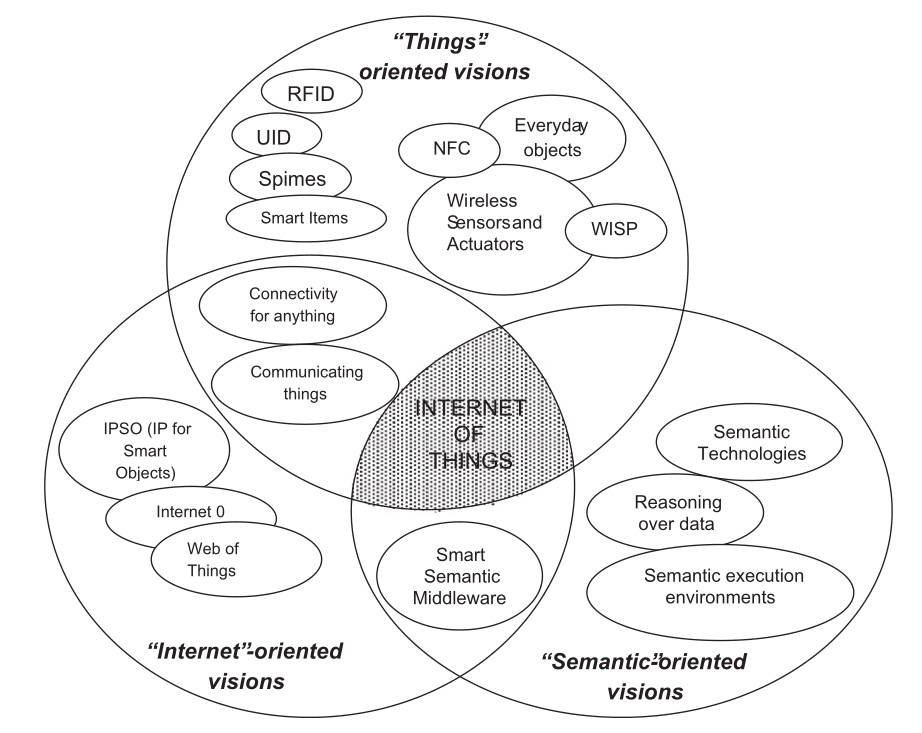
\includegraphics[width=1.0% 图片尺寸,可自行调节
		\textwidth]{fig1.jpg}% 图片名称(图片需与tex文件在同一文件夹)
		\caption{\fontsize{10pt}{15pt}\selectfont “物联网”范式是不同愿景融合的结果。}% 图例
	\end{minipage}
\end{figure}

根据《物联网:将现实世界与数字世界连接起来》的作者,RFID仍然处于推动愿景的技术的前沿。这是RFID成熟、低成本和商业界大力支持的结果。然而,他们表示,广泛的设备、网络和服务技术组合最终将建立物联网。近场通信(NFC)、无线传感器和执行器网络(WSAN)以及RFID被认为是“将现实世界与数字世界联系起来的原子组件”。还值得一提的是,正在开展旨在开发相关平台的重大项目,如WISP(无线识别和传感平台)项目。

《物联网:将现实世界与数字世界连接起来》中的这一点并不是唯一一个明确表示超越RFID的“以信息为导向”的愿景。联合国提出了另一个方案,在2005年突尼斯会议上预测了物联网的到来。一份联合国报告指出,一个无处不在的新时代即将到来,在这个时代,人类可能会成为流量的创造者和接受者,互联网带来的变化将与日常物品联网所带来的变化相比相形见绌。

同样,其他相关机构也强调了物联网主要关注“物”的概念,而全面部署的道路必须从增强物的智能开始。这就是为什么在物联网之外出现的一个概念是时间,它被定义为一个对象,可以在其整个生命周期中通过空间和时间进行跟踪,并且将是可持续的、可增强的和唯一可识别的。虽然是理论上的,但时间定义在所谓的智能物品中找到了一些现实世界的实现。这是一种不仅具有一般的无线通信、记忆、加工能力,而且具有新的潜力的传感器。自主和主动行为、上下文感知、协作沟通和细化只是一些必需的能力。

上述定义为国际电联对物联网的愿景铺平了道路,根据这一愿景:“从随时随地为任何人提供连接,我们现在将为任何事物提供连接”。欧盟委员会的文件和通信中也有类似的愿景,其中最常见的物联网定义涉及“在智能空间中使用智能接口连接和通信的具有身份和虚拟个性的事物,在社会,环境和用户环境中进行连接和通信”。

CASAGRAS联盟还提出了一项物联网愿景声明,其远远超出了单纯的“以RFID为中心”的方法。其成员关注的是“一个事物可以自动与计算机通信并相互提供服务以造福人类的世界”。CASAGRAS联盟(i)提出物联网作为连接虚拟和物理通用对象的全球基础设施的愿景,(ii)强调将现有和不断发展的互联网和网络发展纳入这一愿景的重要性。从这个意义上说,物联网成为部署独立联邦服务和应用程序的自然支持架构,其特点是高度自主的数据捕获、事件传输、网络连接和互操作性。

这个定义在我们所说的“面向物”的愿景和“面向互联网”的愿景之间起着特征结合的作用。

IPSO (IP for Smart Objects)联盟的物联网愿景属于后一类,IPSO是一个由25家创始公司于2008年9月成立的论坛,旨在推广互联网协议作为连接全球智能对象的网络技术。根据IPSO的愿景,IP栈是一种轻型协议,已经连接了大量的通信设备,并运行在微型和电池供电的嵌入式设备上。这保证了IP具有使物联网成为现实的所有品质。通过阅读IPSO白皮书,在6LoWPAN看来,通过明智的IP适应并将IEEE 802.15.4纳入IP架构,物联网范式的全面部署将自动启用。

因特网Ø采用了类似的方法,减少了IP栈的复杂性,从而实现了一种旨在路由“IP over anything”的协议。在一些论坛上,这被视为从设备互联网转向物联网的最明智的方式。根据IPSO和互联网Ø方法,物联网将通过对当前IP的某种简化来部署,以使其适应任何对象,并使这些对象可从任何位置寻址和访问。
如前所述,值得注意的是,“面向语义”的物联网愿景在文献中是可用的。

它们背后的想法是,未来互联网中涉及的项目数量注定会变得非常高。因此,与如何表示、存储、互联、搜索和组织物联网产生的信息相关的问题将变得非常具有挑战性。在这种情况下,语义技术可以发挥关键作用。事实上,这些可以利用适当的建模解决方案来描述事物,对物联网生成的数据进行推理,适应物联网需求的语义执行环境和架构以及可扩展的存储和通信基础设施。

与物联网相关的另一个愿景是所谓的“物联网”,根据该愿景,Web标准被重新用于连接并集成到包含嵌入式设备或计算机的日常生活对象中。


\section{支持技术}
通过集成几种使能技术,可以将物联网概念实现到现实世界中。在本节中,我们将讨论最相关的问题。
请注意,我们的目的不是提供每种技术的全面调查。我们的主要目标是提供它们在物联网中可能扮演的角色的图片。感兴趣的读者可以找到每种特定技术的技术出版物的参考资料。
\subsection{识别、传感和通信技术}
长期以来,“任何时间、任何地点、任何媒体”一直是推动通信技术进步的愿景。在这种情况下,无线技术发挥了关键作用,今天无线电与人类之间的比例接近1比1。

然而,收音机的体积、重量、能源消耗和成本的减少可以把我们带到一个新的时代,在这个时代,上述比例增加了几个数量级。
这将使我们能够将无线电集成到几乎所有对象中,从而将世界“任何东西”添加到上述愿景中,从而导致物联网概念。

在这种情况下,物联网的关键组件将是RFID系统,它由一个或多个读取器和多个RFID标签组成。标签以唯一标识符为特征,并应用于对象(甚至是人或动物)。阅读器通过生成适当的信号来触发标签传输,该信号表示对周围区域可能存在的标签的查询以及对其id的接收。因此,RFID系统可以用来实时监控物体,而不需要在视线范围内;这允许将真实世界映射到虚拟世界。因此,它们可以用于非常广泛的应用场景,从物流到电子医疗和安全。

从物理角度来看,RFID标签是一个附着在天线(用于接收读取器信号和传输标签ID)上的小微芯片1,通常类似于不干胶贴纸。尺寸可以非常小:日立开发了一种尺寸为$0.4mm \times0.4mm\times0.15mm$的标签。

通常,RFID标签是无源的,也就是说,它们没有板载电源,并且从附近的RFID读取器传输的查询信号中获取传输其ID所需的能量。实际上,该信号通过感应产生电流进入标签天线,并利用该电流为微芯片供电,微芯片将传输标签ID。通常,这种系统的增益(读取器接收到的信号功率除以同一读取器发送的信号功率)非常低。然而,由于读取器使用了高度定向的天线,标签ID可以在长达几米的无线电范围内正确接收。传输可以发生在几个频带中,从124 - 135千赫的低频(LF)到860 - 960兆赫的超高频(UHF),这些频带具有最长的范围。

然而,也有RFID标签由电池供电。在这种情况下,我们可以区分半被动和主动RFID标签。在半无源射频识别中,电池在接收读取器信号的同时为微芯片供电(无线电由读取器信号收集的能量供电)。不同的是,在有源射频识别中,电池也为信号的传输提供动力。显然,有源标签的无线电覆盖范围是最高的,即使这是以更高的生产成本为代价实现的。

传感器网络也将在物联网中发挥至关重要的作用。
事实上,它们可以与RFID系统配合,更好地跟踪事物的状态,即它们的位置、温度、运动等。因此,它们可以增强对特定环境的感知,从而在物理世界和数字世界之间充当进一步的桥梁。在环境监测、电子健康、智能交通系统、军事和工业工厂监测等多个应用场景中提出了工作方案。

传感器网络由一定数量(可能非常高)的以无线多跳方式通信的传感节点组成。通常,节点将它们的感知结果报告给少数(在大多数情况下,只有一个)称为sink的特殊节点。近年来,关于传感器网络的大量科学文献已经产生,解决了协议栈各层的几个问题。所提出的解决方案的设计目标是能源效率(在大多数涉及传感器网络的场景中,这是最稀缺的资源)、可扩展性(节点数量可能非常高)、可靠性(网络可能用于报告紧急报警事件)和鲁棒性(传感器节点可能由于多种原因而发生故障)。

如今,大多数商用无线传感器网络解决方案都基于IEEE 802.15.4标准,该标准定义了无线个人局域网(WPAN)中低功耗、低比特率通信的物理层和MAC层。IEEE 802.15.4不包括协议栈更高层的规范,而这是传感器节点无缝集成到互联网中所必需的。这是一项艰巨的任务,原因有很多,最重要的原因如下:

1、传感器网络可能由非常多的节点组成。这将导致明显的问题,因为今天IP地址的可用性很少。

2、IEEE 802.15.4中最大的物理层数据包有127字节;在媒体访问控制层得到的最大帧大小为102字节,根据所使用的链路层安全算法,可以进一步减小。与典型的IP包大小相比,这样的大小太小了。

3、在许多情况下,传感器节点大部分时间处于睡眠模式以节省能量,并且在此期间无法通信。这对于IP网络来说绝对是异常的。

将传感技术集成到无源RFID标签中,将使许多全新的应用能够进入物联网环境,特别是进入电子医疗领域。
最近,在这个方向上提出了几种解决方案。例如,英特尔实验室正在开展WISP项目,以开发无线识别和传感平台(WISP)。wisp由标准RFID读取器供电和读取,从读取器的查询信号中获取能量。wisp已被用于测量特定环境中的量,如光、温度、加速度、应变和液位。

传感RFID系统将允许构建RFID传感器网络,该网络由小型的基于RFID的传感和计算设备以及RFID读取器组成,RFID读取器是传感RFID标签产生的数据的接收器,并为网络运行提供动力。

表1比较了RFID系统(RFID)、无线传感器网络(WSN)和RFID传感器网络(RSN)的特性。观察到的主要优点:

1、RFID系统体积小,成本低。此外,它们的寿命不受电池持续时间的限制;

2、无线传感器网络是高无线电覆盖和通信范式,不需要阅读器的存在(通信是点对点的,而其他类型的系统是不对称的);

3、RFID传感器网络是在无源系统中支持传感、计算和通信能力的可能性。

\subsection{中间件}
中间件是介于技术层和应用层之间的一个软件层或一组子层。它隐藏不同技术细节的功能对于免除程序员与她/他的关注点不直接相关的问题至关重要,即物联网基础设施支持的特定应用程序的开发。中间件在过去几年中变得越来越重要,因为它在简化新服务的开发和将遗留技术集成到新服务中发挥着重要作用。这使程序员无法准确了解下层所采用的各种技术。

正如在其他环境中发生的那样,过去几年为物联网提出的中间件体系结构通常遵循面向服务的体系结构(SOA)方法。
采用SOA原则可以将复杂的单片系统分解为由更简单且定义良好的组件组成的生态系统。公共接口和标准协议的使用提供了企业系统的水平视图。
因此,SOA支持的业务流程的开发是设计协调服务工作流过程的结果,这些服务最终与对象操作相关联。这促进了企业各部分之间的互动,并减少了适应市场演变所带来的变化所需的时间。SOA方法还允许软件和硬件重用,因为它不为服务实现强加特定的技术。

\begin{figure}[H]% 插入一张图片,H表示浮动环境下的here
	\centering
	\begin{minipage}{0.83\textwidth}% 小页面尺寸,可自行调节
		\centering
		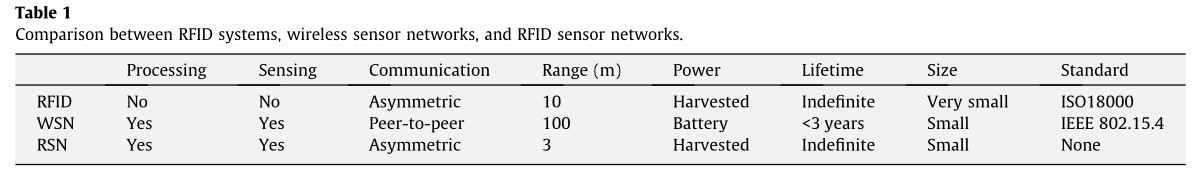
\includegraphics[width=1.0% 图片尺寸,可自行调节
		\textwidth]{fig2.jpg}% 图片名称(图片需与tex文件在同一文件夹)
	\end{minipage}
\end{figure}

SOA方法的优势在大多数物联网中间件解决方案的研究中得到了认可。虽然缺乏普遍接受的分层体系结构,但所提出的解决方案本质上面临相同的问题,即抽象设备功能和通信功能,为服务组合提供一组公共服务和环境。这些共同的目标导致了如图2所示的中间件草图的定义。它试图包含过去处理物联网中间件问题的作品中解决的所有功能。它与中提出的方案非常相似,该方案以完整和集成的体系结构方法解决中间件问题。它依赖于第3.2.1-3.2.5节中解释的层。

\subsubsection{应用程序}
应用程序位于体系结构的顶部,将系统的所有功能导出给最终用户。实际上,这一层不被认为是中间件的一部分,而是利用中间件层的所有功能。
通过使用标准的web服务协议和服务组合技术,应用程序可以实现分布式系统与应用程序之间的完美集成。
\subsubsection{服务组合}
这是基于soa的中间件体系结构之上的公共层。它为网络对象提供的单个服务的组合提供功能,以构建特定的应用程序。在这一层没有设备的概念,唯一可见的资产是服务。对服务环境的一个重要认识是拥有所有当前连接的服务实例的存储库,这些实例在运行时执行以构建组合服务。创建和管理复杂服务背后的逻辑可以使用工作流语言,用业务流程的工作流来表示。在这种情况下,通常的选择是采用标准语言,如业务流程执行语言(BPEL)和Jolie。工作流语言定义了通过使用Web服务定义语言(WSDL)定义的Web服务操作与外部实体交互的业务流程。工作流可以嵌套,因此可以从另一个工作流内部调用工作流。复杂流程的创建可以表示为由单个组件执行的一系列协调操作。

\begin{figure}[H]% 插入一张图片,H表示浮动环境下的here
	\centering
	\begin{minipage}{0.6\textwidth}% 小页面尺寸,可自行调节
		\centering
		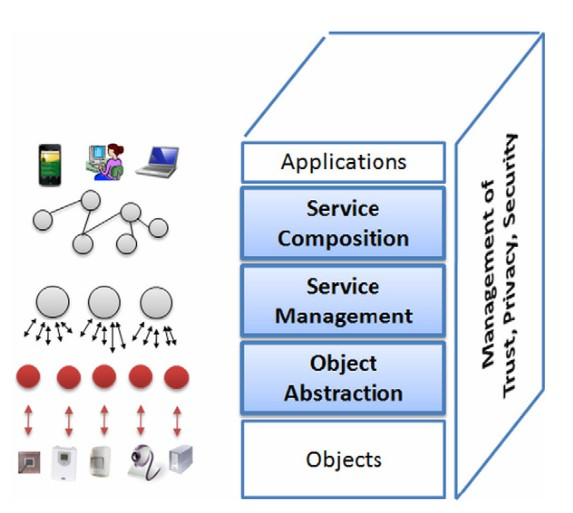
\includegraphics[width=1.0% 图片尺寸,可自行调节
		\textwidth]{fig3.jpg}% 图片名称(图片需与tex文件在同一文件夹)
		\caption{\fontsize{10pt}{15pt}\selectfont 物联网中间件的基于soa的架构。}% 图例
	\end{minipage}
\end{figure}

\subsubsection{服务管理}
这一层提供了每个对象可用的主要功能,并允许在物联网场景中对其进行管理。一组基本的服务包括:对象动态发现、状态监视和服务配置。在这一层,一些中间件建议包括与QoS管理和锁管理相关的扩展功能集,以及一些语义功能(例如,警察和上下文管理)。这一层可能支持在运行时远程部署新服务,以满足应用程序的需求。在这一层构建了一个服务存储库,以便知道哪个是与网络中每个对象相关联的服务目录。然后,上层可以通过连接这一层提供的服务来组合复杂的服务。
\subsubsection{对象抽象}
物联网依赖于一组庞大而异构的对象,每个对象都提供通过自己的方言访问的特定功能。因此,需要一种抽象层,该抽象层能够用公共语言和过程来协调对不同设备的访问。因此,除非设备在IP网络上提供可发现的web服务,否则需要引入包装层,该包装层由两个主要子层组成:接口和通信子层。第一个提供了一个web接口,通过标准web服务接口公开了可用的方法,并负责管理与外部世界通信中涉及的所有传入/传出消息传递操作。第二子层实现web服务方法背后的逻辑,并将这些方法转换为一组特定于设备的命令,以与真实世界的对象通信。

一些工作提出在设备中嵌入TCP/IP堆栈,如TinyTCP、mIP和IwIP(见和本文的参考文献),为嵌入式应用程序提供类似套接字的接口。然后可以将嵌入式web服务器集成到对象中,执行该对象抽象层的功能。然而,这种包装功能通常是通过代理提供的,然后代理负责打开与设备控制台的通信套接字,并通过使用不同的通信语言向其发送所有命令。
然后,它负责将其转换为标准web服务语言,有时还负责详细说明请求,以降低终端设备所需操作的复杂性。

\subsubsection{信任、隐私和安全管理}
在我们的生活中部署对象的自动通信对我们的未来构成了危险。事实上,在用户看不见的情况下,我们的个人设备、衣服和杂货中嵌入的RFID标签可能会在不知不觉中被触发,以回复他们的ID和其他信息。这有可能实现一种监控机制,这种机制将渗透到我们生活的大部分领域。然后,中间件必须包括与所有交换数据的信任、隐私和安全管理相关的功能。相关功能可以建立在先前功能的一个特定层上,也可以(更频繁地发生)以不影响系统性能或引入过度开销的方式分布在整个堆栈中,从对象抽象到服务组合。

虽然大多数提出的中间件解决方案都使用了SOA方法,但其他一些解决方案则采用了不同的方法,尤其是针对特定场景(目标应用程序、特定对象集或有限的地理场景)开发的中间件。一个引人注目的项目是Fosstrak项目,该项目专门专注于RFID相关应用的管理。它是一个开源RFID基础设施,实现EPC网络规范中定义的接口。它提供以下与RFID管理相关的服务:数据传播、数据聚合、数据过滤、写入标签、从外部传感器触发RFID读取器、故障和配置管理、数据解释、共享RFID触发的业务事件、查找和目录服务、标签标识符管理和隐私。所有这些功能都可用于应用层,以简化RFID相关服务的部署。在中,作者提出了另一种与RFID相关的中间件,它依赖于三个功能:标签、地点和风景管理器。
第一个允许用户将每个标签与一个对象相关联;第二支持创建和编辑与RFID天线相关联的位置信息;第三个用于将天线收集的事件与开发的相关应用程序相结合。

e-SENSE项目中提出了另一种不遵循SOA方法的体系结构,该项目专注于通过无线传感器网络捕获环境智能的相关问题。所提出的体系结构分为四个逻辑子系统,即应用程序、管理、中间件和连接子系统。
每个子系统包括各种协议和控制实体,它们在服务接入点向其他子系统提供广泛的服务和功能。整个堆栈在全功能传感器节点和网关节点中实现;而功能减少的传感器节点具有较少的功能。在e-SENSE愿景中,中间件子系统的唯一目的是开发和处理基础设施,在该基础设施中,节点感测到的信息以分布式方式进行处理,并且在必要时,通过网关将结果传输到执行节点和/或固定基础设施。我们分配给中间件的其他功能如图2所示。2属于其他组件和层。UbiSec\&Sens项目还旨在为中大型无线传感器网络定义一个全面的架构,特别关注安全问题,以便为所有应用程序提供一个可信和安全的环境。该体系结构中的中间件层主要集中在:(i)随着时间和某些区域对收集的环境数据进行安全的长期日志记录(TinyPEDS),(ii)为网络中的节点提供共享内存抽象的功能(TinyDSM),(iii)为无线传感器网络实现分布式信息存储和收集(DISC)协议。

\section{应用}
物联网提供的潜力使大量应用程序的开发成为可能,其中只有很小一部分目前可供我们的社会使用。
在许多领域和环境中,新的应用程序可能会改善我们的生活质量:在家里,旅行时,生病时,工作时,慢跑时和在健身房,仅举几例。这些环境现在配备的对象只有原始智能,大多数时候没有任何通信能力。赋予这些对象相互通信的可能性,并细化从周围环境中感知到的信息,意味着可以部署非常广泛的应用程序的不同环境。这些可以分为以下几个领域:

1、运输和物流领域。

2、医疗保健领域。

3、智能环境(家庭、办公室、工厂)领域。

4、个人和社会领域。

在可能的应用中,我们可以区分那些直接适用或更接近我们当前生活习惯的应用,以及那些我们目前只能想象的未来应用,因为技术和/或我们的社会还没有为它们的部署做好准备(见图3)。在下面的小节中,我们将对这些类别的中短期应用和一系列未来应用进行回顾。

\begin{figure}[H]% 插入一张图片,H表示浮动环境下的here
	\centering
	\begin{minipage}{0.9\textwidth}% 小页面尺寸,可自行调节
		\centering
		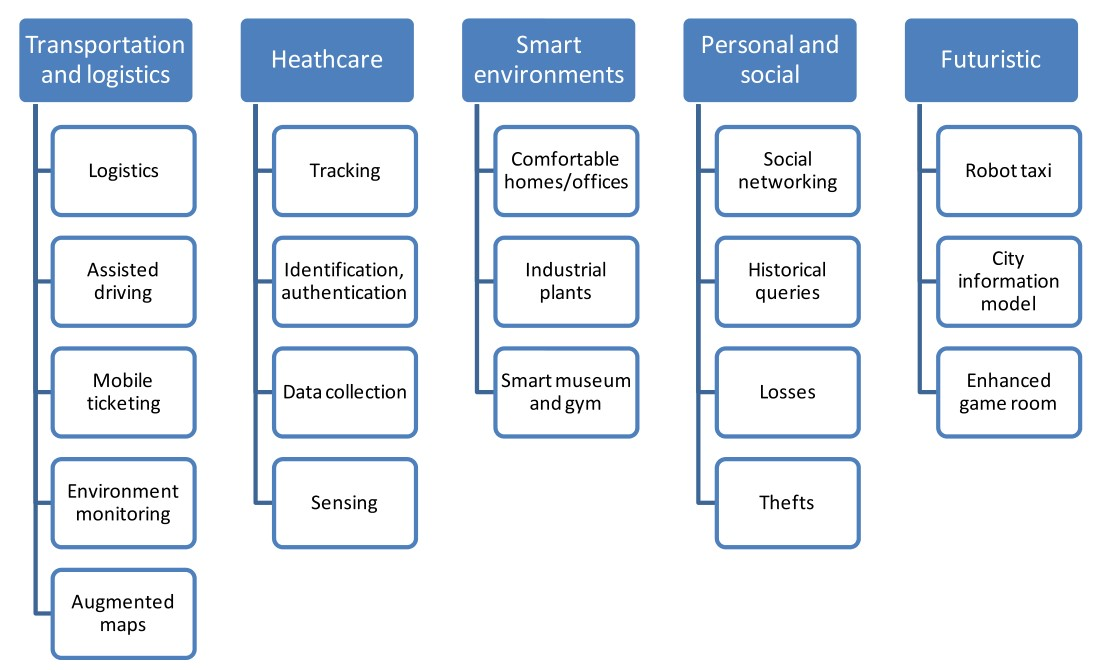
\includegraphics[width=1.0% 图片尺寸,可自行调节
		\textwidth]{fig4.jpg}% 图片名称(图片需与tex文件在同一文件夹)
		\caption{\fontsize{10pt}{15pt}\selectfont 应用领域和相关的主要场景。}% 图例
	\end{minipage}
\end{figure}

\subsection{交通物流领域}
先进的汽车、火车、公共汽车和自行车,以及道路和/或轨道,都越来越多地配备了传感器、执行器和处理能力。道路本身和运输的货物也配备了标签和传感器,这些标签和传感器将重要信息发送给交通控制站点和运输车辆,以便更好地安排交通,帮助管理仓库,为游客提供适当的运输信息,并监控运输货物的状态。下面,描述了在运输和物流领域的主要应用。
\subsubsection{后勤学}
基于实时信息处理技术
RFID和NFC几乎可以实现实时监控
供应链的每一个环节,从商品到
标识、原材料采购、生产、运输、仓储、半成品及成品配送、销售、退货处理及售后服务。还可以及时、及时、准确地获取产品相关信息,使企业乃至整个供应链在最短的时间内对复杂多变的市场做出反应。应用结果是,传统企业从客户需求到商品供应的反应时间为120天,而利用这些技术的先进企业(如沃尔玛、麦德龙等)只需几天时间,基本可以实现零安全库存工作。此外,实时访问ERP程序有助于店员更好地告知顾客产品的可用性,并为他们提供更多的产品信息。

\subsubsection{辅助驾驶}
配备传感器、执行器和处理能力的汽车、火车和公共汽车以及道路和轨道可以为司机和/或汽车乘客提供重要信息,以实现更好的导航和安全。
防撞系统和危险材料运输监控是两个典型的例子。政府当局也将受益于更准确的关于道路交通形态的资料,以便进行规划。而私人交通工具可以更好地找到正确的路径,并提供适当的交通拥堵和事故信息。货运公司等企业将能够进行更有效的路线优化,从而节省能源。将运输货物的车辆的运动信息与货物的种类和状态信息结合起来,可以提供关于交货时间、交货延误和故障的重要信息。
这些信息也可以与仓库的状态相结合,以便自动填充杂志。

\subsubsection{移动票务}
提供有关运输服务的信息(描述、成本、时间表)的海报或面板可以配备NFC标签、视觉标记和数字标识符。然后,用户可以通过将手机悬停在NFC标签上,或者将手机指向视觉标记,从网络上获得关于几类选项的信息。手机自动从相关的网络服务获取信息(车站、乘客人数、费用、可用座位和服务类型),并允许用户购买相关的车票。
\subsubsection{监测环境参数}
易腐食品,如水果、新鲜的农产品、肉类和乳制品是我们营养的重要组成部分。从生产到消费地点覆盖数千公里甚至更远,在运输过程中需要监测保存状态(温度、湿度、冲击),以避免质量水平的不确定性,从而做出分销决策。普适计算和传感器技术为提高食品供应链的效率提供了巨大的潜力。
\subsubsection{增强地图}
旅游地图可以配备标签,允许配备nfc的手机浏览地图,并自动调用网络服务,提供与用户感兴趣的地区有关的酒店、餐馆、纪念碑和事件的信息。有一组物理移动交互(PMI)技术可以用来增强地图信息:

1、在标签的可读范围内悬停,以便在手机屏幕上显示有关该标记的附加信息;

2、当标签处于悬停状态时,通过按特定的键来选择/取消选择标签;

3、多种选择/取消选择不同的标签;

4、通过选择多边形中划分感兴趣区域的标记来绘制多边形;

5、拾取和丢弃,因此使用手机“拾取”的选定标记可以丢弃在感兴趣的行程中;

6、鼠标悬停标记时显示上下文菜单。

\subsection{医疗保健领域}
物联网技术为医疗保健领域提供了许多好处,由此产生的应用主要可以分为:跟踪物体和人员(工作人员和患者),人员识别和认证,自动数据收集和传感。
\subsubsection{追踪}
跟踪是一种旨在识别运动中的人或物体的功能。这既包括实时位置跟踪,例如用于改善医院工作流程的病人流量监测,也包括通过阻塞点(例如进入指定区域)的运动跟踪。对于资产,跟踪最常应用于连续的库存位置跟踪(例如维护,需要时的可用性和使用监测),以及用于防止手术期间遗留的材料跟踪,例如标本和血液制品。
\subsubsection{识别和认证}
它包括患者识别,以减少对患者有害的事件(例如错误的药物/剂量/时间/程序),全面和最新的电子医疗记录维护(包括在住院和门诊设置中),以及医院的婴儿识别,以防止不匹配。对于员工而言,身份识别和认证最常用于授予访问权限,并通过解决患者安全问题来提高员工士气。就资产而言,识别和认证主要用于满足安全程序的要求,以避免重要工具和产品被盗或丢失。
\subsubsection{数据收集}
自动数据收集和传输主要是为了减少表单处理时间、流程自动化(包括数据输入和收集错误)、自动化护理和流程审计以及医疗库存管理。该功能还涉及将RFID技术与设施内的其他健康信息和临床应用技术以及跨提供者和地点的此类网络的潜在扩展集成在一起。
\subsubsection{传感}
传感器设备能够实现以患者为中心的功能,特别是诊断患者病情,提供有关患者健康指标的实时信息。
应用程序领域包括不同的远程医疗解决方案,监控患者对药物团处方的依从性,并为患者的健康状况发出警报。在这种情况下,传感器可以应用于住院和门诊护理。基于异构无线接入的远程患者监测系统可以部署到任何地方的患者,通过集成多种无线技术来支持患者移动时的连续生物信号监测。
\subsection{智能环境领域}
智能环境是指通过包含对象的智能使其“就业”变得轻松舒适,无论是办公室,家庭,工业工厂还是休闲环境。
\subsubsection{舒适的家和办公室}
分布在家庭和办公室的传感器和执行器可以在几个方面使我们的生活更舒适:房间供暖可以根据我们的喜好和天气进行调整;房间的照明可以根据一天中的时间变化;适当的监控和报警系统可避免家庭事故;当不需要时,自动关闭电气设备可以节省能源。例如,我们可以考虑使用动态变化的能源价格来影响整体能源消耗的能源供应商,以一种平滑负荷峰值的方式。自动化逻辑可以通过观察由外部web服务提供并根据当前能源生产和消耗设置的价格何时便宜,并考虑家中每个电器(电池充电器、冰箱、烤箱)的具体要求来优化全天的功耗成本。
\subsubsection{工厂}
通过大量部署与生产部件相关的RFID标签,智能环境还有助于提高工业工厂的自动化程度。在一般情况下,当生产部件到达加工点时,RFID阅读器读取标签。阅读器生成一个事件,其中包含所有必要的数据,如RFID号码,并存储在网络上。机器/机器人收到此事件的通知(因为它已经订阅了服务),并拿起生产部件。通过匹配来自企业系统和RFID标签的数据,它知道如何进一步处理该部件。与此同时,安装在机器上的无线传感器监测振动,如果超过特定阈值,就会引发事件,立即停止过程(质量控制)。一旦这种紧急事件被传播,使用它的设备就会做出相应的反应。机器人收到紧急关机事件,立即停止运行。工厂经理还可以立即看到所谓的企业资源规划(ERP)订单的状态、生产进度、设备状态,以及所有要素的全局视图,以及由于车间设备故障导致的生产线延迟可能产生的副作用。
\subsubsection{智能博物馆和健身房}
在智能休闲环境方面,博物馆和健身房是物联网技术可以最大限度地利用其设施的两个代表性例子。例如,在博物馆里,建筑里的展览可能会唤起不同的历史时期(埃及时期或冰河时期),这些时期的气候条件大相径庭。建筑根据这些条件进行局部调整,同时也考虑到室外条件。在健身房,私人教练可以将每位学员的锻炼档案上传到训练机器上,然后机器通过RFID标签自动识别学员。在整个训练过程中监测健康参数,并检查报告的值,以确定受训者是否训练过度,或者在进行练习时是否过于放松。
\subsection{个人和社会领域}
属于这个领域的应用程序是那些允许用户与其他人进行交互以维护和建立社会关系的应用程序。事实上,一些事情可能会自动触发信息传递给朋友,让他们知道我们正在做什么或我们过去做过什么,比如从家里/办公室搬到家里/办公室,旅行,遇到一些共同的伙伴或踢足球。以下是主要的应用。
\subsubsection{社交网络}
该应用程序与在社交网络门户网站(如Twitter和Plazes)中自动更新有关我们的社交活动的信息有关。我们可能会想到rfid,它产生关于人和地点的事件,为用户提供社交网络中的实时更新,然后将其收集并上传到社交网络网站。
应用程序用户界面显示好友初步定义的事件提要,用户可以控制好友列表以及向哪些好友公开哪些事件。
\subsubsection{历史查询}
对对象和事件数据的历史查询让用户可以研究一段时间内他们活动的趋势。这对于支持长期活动(如业务项目和协作)的应用程序非常有用。可以构建一个数字日记应用程序,记录和显示事件,例如在Google Calendar中供以后阅读。通过这种方式,用户可以回顾他们的日记,看看他们是如何度过时间的,以及和谁一起度过的。还可以使用Google Charts API自动生成历史趋势图,以显示在任意时间段内他们在哪里、如何以及与谁或什么人一起度过时间。
\subsubsection{损失}
搜索引擎是一种工具,可以帮助我们找到那些我们不记得放在哪里的东西。最简单的基于web的RFID应用程序是一个物品搜索引擎,它允许用户查看其标记对象的最后记录位置或搜索特定对象的位置。这个应用程序的一个更主动的扩展利用用户定义的事件,在最后记录的对象位置与某些条件匹配时通知用户。
\subsubsection{盗窃}
与上一个类似的应用程序可能允许用户知道某些对象是否从受限区域(所有者的房屋或办公室)移动,这将表明该对象正在被盗。在这种情况下,必须立即将事件通知给所有者和/或保安人员。例如,当被盗物品(如笔记本电脑、钱包或装饰品)未经任何授权离开建筑物时,应用程序可以向用户发送短信。
\subsection{未来应用领域}
前面章节中描述的应用程序是现实的,因为它们要么已经部署,要么可以在短/中期内实现,因为所需的技术已经可用。除此之外,我们还可以设想许多其他的应用,我们在这里将其定义为未来的应用,因为这些应用依赖于一些(通信、传感、材料和/或工业过程)技术,这些技术要么尚未出现,要么实现起来仍然过于复杂。就所需的研究和潜在影响而言,这些应用程序甚至更有趣。SENSEI FP7项目提供了对这类应用程序的有趣分析,我们从中选取了三个最吸引人的应用程序。
\subsubsection{机器人出租车}
在未来的城市中,机器人出租车聚集在一起,成群结队地移动,及时有效地为需要的地方提供服务。机器人出租车对城市的实时交通状况做出反应,并进行校准,以减少城市瓶颈处的拥堵,并为最常用的接送区域提供服务。不管有没有人类驾驶员,它们都能以最佳速度在车流中穿梭,通过接近传感器避免事故的发生。接近传感器通过磁力将它们与道路上的其他物体隔离开来。你可以在路边用手机对着他们,或者用手势招呼他们。通过GPS自动跟踪用户的位置,用户只需在详细的地图上指出特定地点,就可以要求出租车在特定时间到达特定地点。在极少情况下无人使用的情况下,这些出租车会前往“维修站”,在那里,它们会自动把自己塞进装有传感器的狭小隔间里,在那里,执行器会启动充电电池,执行简单的维护任务,并清洁汽车。进站之间相互通信,以确保没有过度或不足的利用。
\subsubsection{城市信息模型}
城市信息模型(CIM)的概念是基于这样一个概念,即每个建筑和城市结构的状态和性能——比如人行道、自行车道和下水道、铁路线和公交走廊等较重的基础设施——由市政府持续监控,并通过一系列api提供给第三方,尽管有些信息是保密的。因此,除非与CIM兼容,否则任何东西都不能合法建造。设施管理服务彼此之间和CIM之间进行通信,以最具成本效益和资源效率的方式共享能源。
它们之间会自动进行剩余能源的交易,并计算出与供需相匹配的价格。
从这个意义上说,规划和设计是一个持续的社会过程,其中每个项目的表现都是实时报告的,并与其他项目进行比较。
可以推断出人口的变化、移动模式、环境表现以及产品和建筑的整体效率。
\subsubsection{增强型游戏室}
增强型游戏室和玩家都配备了各种设备,可以感应位置、运动、加速度、湿度、温度、噪音、语音、视觉信息、心率和血压。房间使用这些信息来测量兴奋和能量水平,以便根据玩家的状态控制游戏活动。房间里还放置了各种各样的物体,游戏的目的是在不接触地板的情况下从一个物体爬到另一个物体。跳远和难以到达的地方都会获得积分。游戏还在壁挂式屏幕上放置一个目标。谁先到达目标,谁就赢。当玩家在房间里走来走去时,游戏会记录他们的成就。他们的控制器可以识别房间里物体上的RFID标签。为了得分,他们必须用它触摸物体。随着比赛的进行,系统逐渐增加了难度。
起初,他们必须到达的物体就在附近,而且很容易到达。在某些时候,这变得太难了,两名球员都必须用脚触地。然后游戏发出巨大的噪音,表明这是错误的。房间现在注意到一名球员比另一名球员高一点,速度也快一点,所以它开始把物体放得离他更近一点,这样他就可以跟上了。然后,游戏根据玩家的成绩调整难度水平和目标,以保持控制台通过传感设备感知到的高兴奋水平。
\section{未决问题}
尽管第3节中描述的使能技术使物联网概念变得可行,但仍需要大量的研究工作。在本节中,我们首先回顾了在不同物联网相关技术上正在进行的标准化活动(第5.1节)。其次,我们展示了需要解决的最重要的研究问题,以满足物联网场景的特征要求。更具体地说,在第5.2节中,我们重点讨论了解决和联网问题,而在第5.3节中我们描述了与安全和隐私相关的问题。

在表2中,我们总结了开放的研究问题,它们对物联网场景特别重要的原因,以及将详细讨论这些问题的部分。

\begin{figure}[H]% 插入一张图片,H表示浮动环境下的here
	\centering
	\begin{minipage}{1\textwidth}% 小页面尺寸,可自行调节
		\centering
		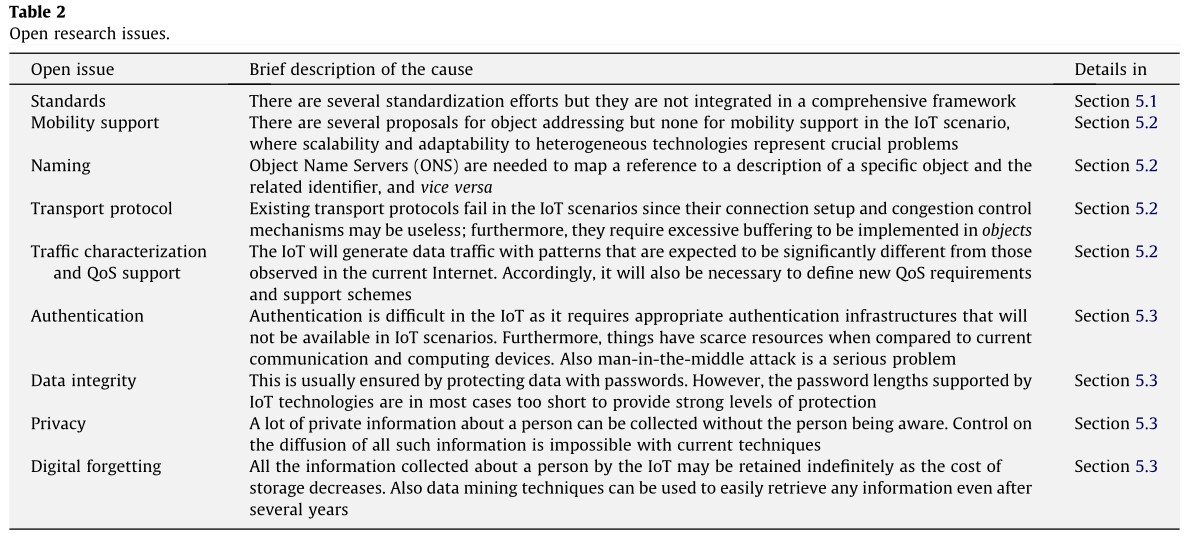
\includegraphics[width=1.0% 图片尺寸,可自行调节
		\textwidth]{fig5.jpg}% 图片名称(图片需与tex文件在同一文件夹)
	\end{minipage}
\end{figure}

\subsection{标准化活动}
科学界对物联网范式的全面部署和标准化做出了一些贡献。其中,最相关的是由分散在世界各地的自动识别实验室的不同部门提供的,由欧盟委员会和欧洲标准组织(ETSI, CEN, CENELEC等),由其国际同行(ISO, ITU)以及其他标准机构和联盟(IETF, EPCglobal等)提供。特别期望来自欧洲电信标准协会(ETSI)的机器对机器工作组和一些互联网工程任务组(IETF)工作组的输入。旨在使IPv6协议兼容低容量设备的LoWPAN和对未来互联网场景路由问题更感兴趣的ROLL是最佳候选方案。

在表3中,我们从标准的目标、标准化过程的状态、通信范围、数据速率和设备成本等方面总结了主要标准的基本特征。在表中,我们突出显示了本节中详细讨论的标准。

关于RFID技术,目前由于标准化的分散努力而放慢了速度,标准化主要集中在两个主要领域:RFID频率和阅读器-标签(标签-阅读器)通信协议,标签和标签上的数据格式。处理RFID系统的主要标准化机构是EPCglobal、ETSI和ISO。

更具体地说,EPCglobal是全球非营利标准组织GS1的子公司。它的主要目的是支持全球采用每个标签的唯一标识符,即电子产品代码(EPC),以及相关的行业驱动标准。提出“EPCglobal架构框架”的建议是EPCglobal的一个目标,与专家社区和一些组织共享,包括自动识别实验室、GS1全球办公室、GS1成员组织、政府机构和非政府组织(ngo)。有趣的结果已经出现。

至于欧盟委员会的努力,可能对未来RFID标准化进程影响最大的事件无疑是所谓的“RFID实施非正式工作组”的正式成立。这是由利益相关者(行业,运营商,欧洲标准组织,民间社会组织,数据保护当局等)组成的,要求“熟悉RFID的一般情况,数据保护指令和RFID建议”。

其中一个利益相关者,CEN(欧洲标准化委员会),虽然没有开展任何专门与物联网相关的活动,但对RFID向物联网的发展感兴趣。在其工作组(WG)中,与物联网最相关的是WG 1-4条形码,WG 5 RFID和全球RFID互操作性标准论坛(GRIFS)。后者是一个由GS1、ETSI和CEN协调的为期两年的项目,旨在定义与RFID使用的物理对象(读取器、标签、传感器)、通信基础设施、频谱、影响RFID的隐私和安全问题相关的标准。

与这些项目不同,ISO侧重于技术问题,如使用的频率、调制方案和防碰撞协议。

就物联网范式而言,ETSI(欧洲电信标准协会,负责制定全球适用的ICT相关标准)正在开展一项非常有趣的标准化工作。事实上,在ETSI内部,成立了机器对机器(M2M)技术委员会,目的是开展与M2M系统和传感器网络相关的标准化活动(从物联网的角度来看)。M2M是物联网的真正领先范例,但它的标准化很少,而市场上的解决方案的多样性使用标准的互联网,蜂窝和Web技术。因此,ETSI M2M委员会的目标包括:开发和维护M2M的端到端架构(背后有端到端IP理念),加强M2M的标准化工作,包括传感器网络集成、命名、寻址、定位、QoS、安全、收费、管理、应用和硬件接口。

\begin{figure}[H]% 插入一张图片,H表示浮动环境下的here
	\centering
	\begin{minipage}{1\textwidth}% 小页面尺寸,可自行调节
		\centering
		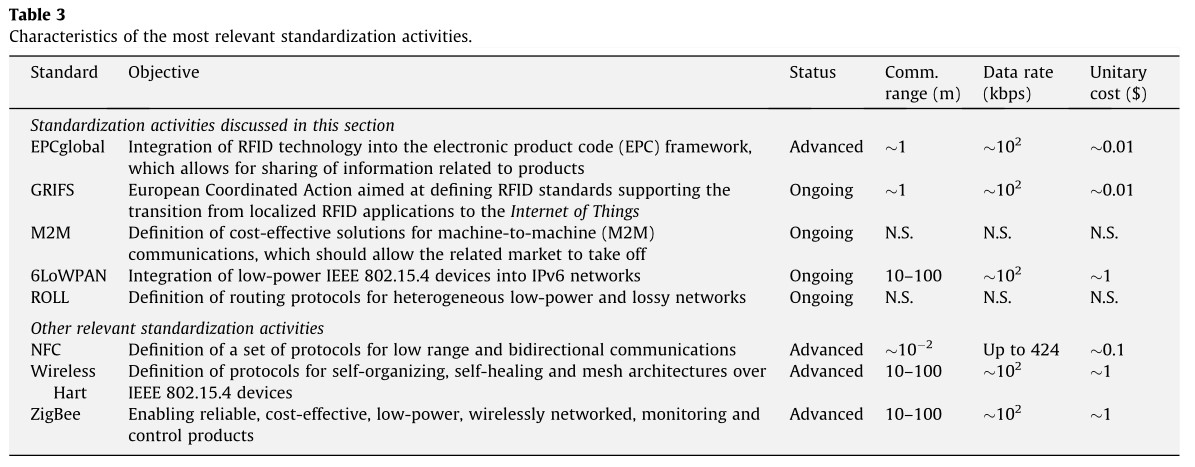
\includegraphics[width=1.0% 图片尺寸,可自行调节
		\textwidth]{fig6.jpg}% 图片名称(图片需与tex文件在同一文件夹)
	\end{minipage}
\end{figure}

至于互联网工程任务组(IETF)与物联网相关的活动,我们可以说,最近低功耗无线个人区域网络(6LoWPAN) IPv6 IETF组诞生了。LoWPAN正在定义一组可用于将传感器节点集成到IPv6网络中的协议。组成6LoWPAN体系结构的核心协议已经被指定,并且已经发布了一些实现该协议套件的商业产品。6LoWPAN工作组目前正在标准轨道(改进报头压缩,6LoWPAN邻居发现)和信息轨道(用例,路由需求)中移动四个互联网草案。

另一个相关的IETF工作组名为低功耗和有损网络路由(ROLL)。它最近产生了RPL(发音为“ripple”)路由协议草案。这将是在低功耗和有损网络(包括6LoWPAN)上路由的基础,它仍然需要大量的贡献才能达到完整的解决方案。

从以上所述,我们清楚地了解到,一个新兴的想法是将物联网标准化视为未来互联网定义和标准化过程的一个组成部分。最近,欧洲物联网研发项目集群(CERP-IoT)做出了这一断言。根据该理论,将不同的事物整合到更广泛的网络中,无论是移动的还是固定的,都将允许它们与未来的互联网互联。

值得指出的是,在上述标准化领域,标准化机构与其他世界范围的利益集团和联盟之间的紧密合作。似乎整个行业都愿意合作实现物联网。IPSO,还有ZigBee联盟、IETF和IEEE都在朝着IP标准集成的同一方向努力.
\subsection{解决和网络问题}
物联网将包括数量惊人的节点,每个节点都将产生任何授权用户都可以检索的内容,无论她/他的位置如何。这需要有效的解决政策。目前,IPv4协议通过一个4字节的地址来标识每个节点。众所周知,可用的IPv4地址数量正在迅速减少,并将很快达到零。因此,除了IPv4使用的寻址策略外,显然还应该使用其他寻址策略。

在这种情况下,正如我们在5.1节中已经说过的,IPv6寻址已经被提议用于6LoWPAN环境中的低功耗无线通信节点。IPv6地址由128位表示,因此,可以定义1038个地址,这应该足以识别任何值得被寻址的对象。因此,我们可以考虑为网络中包含的所有东西分配一个IPv6地址。然而,由于RFID标签使用64-96位标识符,因此需要解决方案将RFID标签寻址到IPv6网络中。最近,研究人员对RFID标签与IPv6网络的集成进行了研究,并提出了将RFID标识符与IPv6地址集成的方法。例如,在《EPC与IPv6映射机制》中,作者提出使用IPv6地址的64位接口标识符来报告RFID标签标识符,而其他64位网络前缀用于寻址RFID系统和Internet之间的网关。

因此,网关将处理RFID标签产生的消息,这些消息必须离开RFID系统并进入Internet,如下所示。将创建一个新的IPv6报文。它的有效负载将包含由标签生成的消息,而它的源地址将通过连接网关ID(复制到IPv6地址的网络前缀部分)和RFID标签标识符(复制到IPv6地址的接口标识符部分)来创建。类似地,网关将处理来自Internet的IPv6数据包,并将其定向到某个RFID标签,如下所示。代表消息目的地的特定RFID标签将很容易被识别,因为它的标识符被报告到IPv6地址的接口标识符部分;而特定的消息(在大多数情况下表示某个操作的请求)将被通知到相关的RFID读取器。

但是,如果RFID标签标识符是EPCglobal标准所允许的96位长,则不能使用这种方法。为了解决这个问题,在《使用地址管理代理的RFID联网机制》中提出了一种方法,该方法使用一种适当的网络元素,称为agent,将RFID标识符(无论其长度如何)映射为一个64位字段,该字段将用作IPv6地址的接口ID。显然,代理必须更新生成的IPv6地址和RFID标签标识符之间的映射。

使用-RFID和IPv6中说明了一种完全不同的方法,其中RFID消息和报头包含在IPv6数据包有效载荷中,如图4所示。

但是,需要注意的是,在上述所有情况下都不支持RFID移动性。事实上,常见的基本假设是,每个RFID都可以通过网络和RFID系统之间的给定网关到达。

因此,需要适当的机制来支持物联网场景中的移动性。在这种情况下,整个系统将由大量具有极其不同特征的子系统组成。在过去,针对移动性管理提出了几种解决方案;然而,它们在物联网场景中的有效性应该得到证明,因为它们在应用于这种异构环境的可扩展性和适应性方面可能存在问题。为此,重要的是要注意,基于家庭代理(如移动IP)的解决方案可以实现更高的可扩展性,而不是基于家庭位置寄存器(HLR)和访问者位置寄存器(VLR)的解决方案,后者在蜂窝网络中广泛使用。事实上,移动类ip协议不使用中央服务器,而从可伸缩性的角度来看,中央服务器是至关重要的。

另一个问题是获取地址的方式。在传统的互联网中,任何主机地址都是通过查询称为域名服务器(DNS)的适当服务器来识别的。DNSs的目的是从某个输入名称中提供主机的IP地址。在物联网中,通信可能发生在对象之间(或与对象之间),而不是主机之间。因此,必须引入对象名称服务(ONS)的概念,该概念将参考与特定对象的描述和相关RFID标签标识符相关联。事实上,标签标识符被映射到互联网统一参考定位器(URL)中,该URL指向对象的相关信息。在物联网中,ONS应在两个方向上运行,即应能够将指定对象的描述与给定的RFID标签标识符相关联,反之亦然。转换函数并不容易,需要一种适当的服务,称为对象代码映射服务(OCMS)。中报告了OCMS所需的特性,其中建议采用P2P方法来提高可扩展性。然而,请注意,在复杂的操作环境(如物联网)中,OCMS的设计和评估仍然是悬而未决的问题。

\begin{figure}[H]% 插入一张图片,H表示浮动环境下的here
	\centering
	\begin{minipage}{0.83\textwidth}% 小页面尺寸,可自行调节
		\centering
		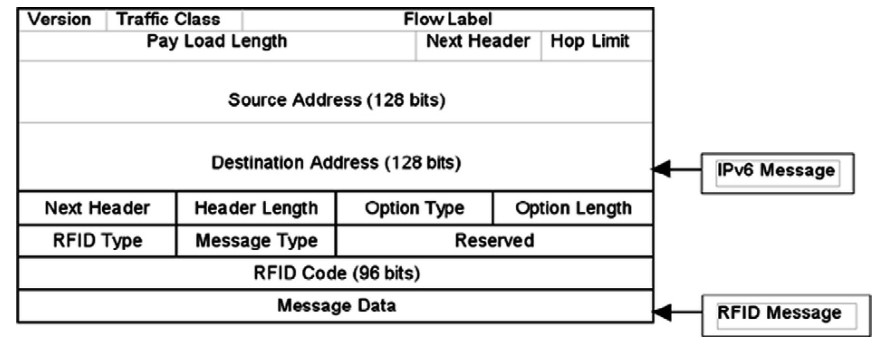
\includegraphics[width=1.0% 图片尺寸,可自行调节
		\textwidth]{fig7.jpg}% 图片名称(图片需与tex文件在同一文件夹)
		\caption{\fontsize{10pt}{15pt}\selectfont 将RFID消息封装到IPv6数据包中。}% 图例
	\end{minipage}
\end{figure}
此外,物联网还需要一个新的传输层概念。传输层的主要目标是保证端到端的可靠性并执行端到端拥塞控制。在传统互联网中,传输层用于可靠通信的协议是传输控制协议(TCP)。很明显,TCP不适合物联网,原因如下:

1、连接设置:TCP是面向连接的,每个会话都以连接设置过程(所谓的三方握手)开始。这是不必要的,因为物联网内的大多数通信将涉及少量数据的交换,因此,设置阶段将持续相当一部分会话时间。此外,连接建立阶段涉及要由终端处理和传输的数据,在大多数情况下,终端在能量和通信资源方面都是有限的,例如传感器节点和RFID标签。

2、拥塞控制:TCP负责执行端到端的拥塞控制。在物联网中,这可能会导致性能问题,因为大多数通信都会利用无线介质,众所周知,无线介质对TCP来说是一个具有挑战性的环境。此外,如果在单个会话中要交换的数据量非常小,则TCP拥塞控制是无用的,因为整个TCP会话将以第一段的传输和随后的相应确认的接收结束。

3、数据缓冲:TCP要求数据存储在源和目的地的内存缓冲区中。事实上,在源数据应该进行缓冲,以便在数据丢失时可以重新传输。在目的地,应该缓冲数据,以便向应用程序提供有序的数据传递。就无电池设备所需的能量而言,这种缓冲器的管理可能过于昂贵。

因此,TCP不能有效地用于物联网中的端到端传输控制。到目前为止,还没有提出物联网的解决方案,因此需要研究贡献。

此外,我们不知道物联网中智能对象交换的流量的特征是什么。然而,研究这些特性是至关重要的,因为它们应该是网络基础设施和协议设计的基础。

因此,关于网络方面的另一个重要研究问题与流量表征有关。众所周知,无线传感器网络中的流量特性在很大程度上取决于应用场景。这不是一个问题,因为人们的兴趣集中在无线传感器网络本身内部的流量上。根据物联网范式,当传感器节点成为整个互联网的一部分时,就会出现复杂情况。事实上,在这种情况下,互联网将被部署用于异构目的的传感器网络生成的大量数据所遍历,因此具有极其不同的流量特性。此外,由于大规模分布式RFID系统的部署仍处于起步阶段,到目前为止还没有研究相关流量的特征,因此,将穿越物联网的流量是完全未知的。

相反,流量的特征非常重要,因为网络提供商有必要规划其基础设施的扩展(如果需要)。

最后,需要将流量特征化和建模与流量需求列表一起设计用于支持服务质量(QoS)的适当解决方案。事实上,如果已经为支持无线传感器网络中的QoS做了一些工作,那么在RFID系统中这个问题仍然完全没有被探索。因此,需要在物联网中的QoS支持领域进行大量的研究。我们相信,机器对机器通信的QoS有几个相似之处。由于近年来已经解决了此类通信,我们可以将其应用于物联网场景,为M2M场景提出的QoS管理方案。显然,这应该只是一个起点,未来应该引入物联网的具体解决方案。
\subsection{安全和隐私}
只要公众不相信物联网不会对隐私造成严重威胁,人们就会抵制物联网。
意大利零售商贝纳通宣布计划为一整套衣服(约1500万个RFID)贴标签后,所有的谈话和抱怨都首次明确证实了这种对物联网技术收集的数据使用的不信任。

公众关注的问题确实可能集中在一定数量的安全和隐私问题上。
\subsubsection{安全}
物联网极易受到攻击,原因有几个。首先,它的组件通常大部分时间都是无人看管的;因此,很容易对他们进行身体攻击。

其次,大多数通信都是无线的,这使得窃听变得极其简单。最后,大多数物联网组件的特点是在能源和计算资源方面能力低下(无源组件尤其如此),因此,它们无法实现支持安全的复杂方案。

更具体地说,与安全相关的主要问题涉及身份验证和数据完整性。身份验证很困难,因为它通常需要适当的身份验证基础设施和服务器,通过与其他节点交换适当的消息来实现其目标。在物联网中,考虑到被动RFID标签无法与认证服务器交换太多消息,这种方法是不可行的。同样的推理也适用于传感器节点(以限制较少的方式)。

在这种情况下,请注意,最近已经为传感器网络提出了几种解决方案。然而,当传感器节点被视为传感器网络的一部分,通过扮演网关角色的一些节点连接到互联网的其余部分时,可以应用现有的解决方案。相反,在物联网场景中,传感器节点必须被视为互联网的节点,因此即使不属于同一传感器网络的节点也有必要对其进行身份验证。

在过去的几年里,已经为RFID系统提出了一些解决方案,然而,如《RFID安全与隐私:一项研究调查》所述,它们都存在严重的问题。

最后,现有的解决方案都无法帮助解决代理攻击问题,也称为中间人攻击。考虑这样一种情况,即节点被用来识别某物或某人,并相应地提供对特定服务或特定区域的访问(例如,考虑电子护照或一些基于RFID的密钥)。图5所示的攻击可以成功执行。

考虑这样的情况:A是想要通过某种RF机制验证其他系统元素的节点,而攻击者想要窃取元素B的身份(请注意,B可以是任何能够计算和通信的物联网元素)。攻击者将定位两个收发器。第一个接近A,我们称之为B0,第二个接近B,我们称其为A0。基本思想是让A相信B0是B,让B相信A0是A。为此,节点B0将把认证节点A接收到的查询信号发送到收发器A0。收发器A0将发送这样的信号,以便B可以接收。注意,A0发送的信号是A发送的信号的精确副本。因此,节点B不可能理解该信号不是由A发送的,因此,它将用其标识进行回复。节点A0接收这样的应答并将其发送到节点B0,节点B0将把它发送到节点A。节点A不能区分这样的应答不是由B发送的,因此,将把收发器B0识别为单元B并相应地提供接入。注意,无论信号是否加密,都可以这样做。

\begin{figure}[H]% 插入一张图片,H表示浮动环境下的here
	\centering
	\begin{minipage}{0.6\textwidth}% 小页面尺寸,可自行调节
		\centering
		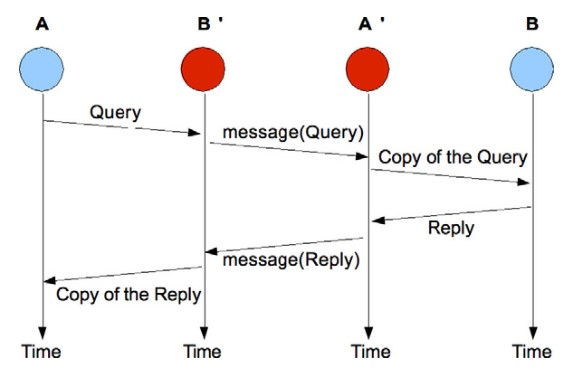
\includegraphics[width=1.0% 图片尺寸,可自行调节
		\textwidth]{fig8.jpg}% 图片名称(图片需与tex文件在同一文件夹)
		\caption{\fontsize{10pt}{15pt}\selectfont 中间人攻击}% 图例
	\end{minipage}
\end{figure}

数据完整性解决方案应确保对手在没有系统检测到更改的情况下无法修改交易中的数据。数据完整性问题在所有传统的计算和通信系统中都得到了广泛的研究,传感器网络也有一些初步结果。然而,当RFID系统集成到互联网中时,会出现新的问题,因为它们大部分时间都是无人看管的。当数据存储在节点中或穿过网络时,对手可以修改数据。为了保护数据免受第一种类型的攻击,在大多数标签技术中都对内存进行了保护,并为无线传感器网络提出了解决方案。例如,EPCglobal Class 1 Generation-2和ISO/IEC 18000–3标签都使用密码保护其内存上的读写操作。事实上,EPCglobal Class 1 Generation-2标签有五个内存区域,每个内存区域都可以通过彼此独立的密码进行读写保护。然而,ISO/18000–3标签定义了指向内存地址的指针,并使用密码保护内存地址较低的所有内存区域。为了保护数据免受第二类攻击,可以根据密钥散列消息认证码(HMAC)方案来保护消息。这是基于标签和消息目的地之间共享的公共密钥,该密钥与哈希函数结合使用以提供身份验证。

观察到,当RFID系统被认为存在严重问题时,为支持数据完整性而提出的上述解决方案。事实上,大多数标签技术支持的密码长度太短,无法提供强大的保护级别。此外,即使支持更长的密码,它们的管理仍然是一项具有挑战性的任务,尤其是当涉及到属于不同组织的实体时,如物联网。

最后,请注意,为支持安全性而提出的所有解决方案都使用了一些加密方法。典型的密码算法在源和目的地都花费了大量的能量和带宽资源。这种解决方案无法应用于物联网,因为它们将包括在能源、通信和计算能力方面受到严重限制的元件(如RFID标签和传感器节点)。因此,需要新的解决方案,能够在资源匮乏的情况下提供令人满意的安全水平。在这种情况下,已经为光对称密钥加密方案提出了一些解决方案。然而,正如我们已经说过的,密钥管理方案仍处于早期阶段(尤其是在RFID的情况下),需要大量的研究工作。
\subsubsection{隐私}
隐私的概念深深植根于我们的文明,在文明国家的所有立法中都得到了承认,正如我们已经说过的,对其保护的担忧已被证明是阻碍物联网技术传播的重要障碍。人们对隐私的担忧确实是有充分理由的。事实上,物联网中完成数据收集、挖掘和供应的方式与我们现在所知道的完全不同,收集个人数据的情况会非常多。

因此,对于人类个人来说,不可能亲自控制其个人信息的披露。

此外,信息存储成本持续下降,目前已接近10-9欧元/字节。

因此,一旦信息产生,很可能会被无限期地保留,这涉及到从人们的角度否认数字遗忘。

由此可见,物联网确实代表了一个个人隐私在多种方面受到严重威胁的环境。此外,虽然在传统的互联网中,隐私问题主要出现在互联网用户(发挥积极作用的个人)身上,但在物联网场景中,即使不使用任何物联网服务的人也会出现隐私问题。

因此,应通过确保个人能够控制正在收集的个人数据、谁在收集这些数据以及何时收集这些数据来保护隐私。此外,所收集的个人数据只能用于支持授权服务提供商的授权服务;最后,上述数据只应存储到严格需要时为止。

例如,考虑第4.3节中描述的关于舒适住宅和办公室的应用场景,并将重点放在几个办公室所在的建筑的情况下。在这种情况下,将在环境中部署一些传感能力,以跟踪人员的位置并相应地控制照明或加热。如果部署跟踪系统只是为了在减少能源消耗的同时提高办公室的舒适度,那么应采用适当的隐私保护政策,以确保:

1、跟踪系统不收集关于个人用户的位置和移动的信息,而只考虑聚合用户(人的位置和运动不应与他们的身份相关联);

2、让人们了解系统跟踪他们行动的范围和方式(让人们了解他们的隐私可能被泄露是至关重要的,也是大多数立法所要求的);

3、由跟踪系统收集的数据应该被处理以控制照明和加热,然后由存储系统删除。

为了处理数据收集过程,在物联网中与人类交互的所有不同子系统中都需要适当的解决方案。例如,在传统互联网服务的背景下,W3C小组定义了隐私偏好平台(P3P),该平台为隐私偏好和策略的描述提供了一种语言,因此,允许基于运行服务的个人信息的需要和用户设置的隐私要求来自动协商与隐私有关的参数。总是在传统互联网服务的背景下,通过对用户终端上运行的应用程序的适当设置,可以容易地检测个人信息被发布的时刻,并且可以通过建立良好的认证程序来识别收集此类数据的实体。

在传感器网络的情况下,该问题变得不可能解决。事实上,进入部署传感器网络的区域的个人无法控制收集到的关于自己的信息。例如,考虑一个由部署在特定区域的摄像头组成的传感器网络。个人避免此类摄像头不拍摄其图像的唯一方法是不进入该区域。在这种情况下,可以减少隐私问题的可能解决方案可能是限制网络在可能损害隐私的细节级别收集数据的能力。

例如,传感器网络可以通过仅报告感测到的个人的大致位置来匿名化数据,并在隐私要求与应用程序所需的细节级别之间进行权衡。关于传感器网络的另一个例子,该传感器网络由用于视频监控目的的摄像机组成。在这种情况下,为了保护人们的隐私,人们的图像可能会被模糊。如果发生了一些事件,那么执法人员可以重建相关人员的图像。

在RFID系统的情况下,问题是双重的。事实上,一方面,RFID标签通常是被动的,并回复读者的查询,而不考虑其所有权的需求。另一方面,攻击者可以窃听标签对另一个授权阅读器的回复。迄今为止提出的第一类问题的解决方案是基于授权读者的身份验证(上面已经讨论过)。然而,这样的解决方案需要能够执行身份验证过程的标签。这涉及更高的成本和身份验证基础设施,正如我们已经说过的,这无法部署在物联网场景中预期的复杂系统中。

因此,最近提出了使用新系统的解决方案,该系统基于用户设置的偏好,代表用户协商隐私。上述系统做出的隐私决定可以通过在无线信道中与不应读取的RFID标签发送的回复发生冲突来强制执行。

如上所述,可以通过加密保护通信来避免RFID系统中攻击者的窃听。然而,这些类型的解决方案仍然允许恶意读取器检测授权读取器扫描的RFID标签的存在。为了解决这个问题,有一种新的解决方案家族,其中读取器传输的信号具有伪噪声的形式。这种噪声信号由RFID标签调制,因此恶意读取器无法检测到其传输。

为了确保收集的个人数据仅用于支持授权提供商的授权服务,已经提出了通常依赖于称为隐私代理的系统的解决方案。代理一方面与用户交互,另一方面与服务交互。因此,它保证提供者只获得严格需要的关于用户的信息。用户可以设置代理的首选项。当传感器网络和RFID系统包括在网络中时,代理在它们和服务之间运行。但是,请注意,在这种情况下,个人无法设置和控制隐私代理所使用的策略。此外,请注意,这种基于隐私代理的解决方案存在可扩展性问题。

最后,关于数字遗忘的研究仍处于起步阶段,因为直到最近才被认为是一个重要问题。事实上,随着存储成本的降低,可以存储的数据量急剧增加。因此,有必要创建定期删除对其生成目的毫无用处的信息的解决方案。因此,未来将开发的新软件工具应该支持这种遗忘功能。例如,最近开发并发布了一些实验性解决方案供公众使用,这些解决方案允许用户在互联网上插入和共享图片和其他类型的文件,并保证这些图片在某个日期过期,之后会被删除(例如,请参阅drop.io和Flickr上的Guest Pass功能)。将此类解决方案移植到物联网环境中并不简单,需要进一步的研究工作。
\section{总结}
互联网极大地改变了我们的生活方式,将人与人之间的互动转移到了从职业生活到社会关系的几个虚拟层面。物联网有可能通过实现与智能对象之间的通信,为这一过程增加一个新的维度,从而实现“实时、任何地方、任何媒体、任何东西”的通信愿景。

为此,我们观察到,物联网应该被视为未来整体互联网的一部分,这可能与我们今天使用的互联网截然不同。事实上,很明显,目前的互联网模式支持主机到主机的通信,并且是围绕主机到主机通信构建的,现在是互联网当前使用的一个限制因素。很明显,互联网主要用于信息的发布和检索(无论这些信息是从哪里发布或检索的),因此,信息应该是通信和网络解决方案的重点。这导致了以数据为中心的网络的概念,直到最近才进行了研究。

根据这样一个概念,数据和相关查询是可自寻址和可自路由的。

从这个角度来看,我们在第5.2节中强调的当前趋势,即为每个物联网元素分配IPv6地址,以便能够从网络的任何其他节点访问它们,看起来更适合传统的互联网模式。因此,互联网的发展可能需要改变上述趋势。

另一个在未来互联网背景下出现的有趣范式是所谓的Web Squared,它是Web 2.0的演变。它旨在将网络和传感技术集成在一起,以丰富提供给用户的内容。这是通过考虑由部署在用户终端中的传感器(麦克风、相机、GPS等)收集的关于用户上下文的信息来获得的。从这个角度来看,Web Squared可以被视为在物联网上运行的应用程序之一,就像今天Web是在互联网上运行的(重要)应用程序一样。

在本文中,我们调查了物联网最重要的方面,重点是正在做什么以及需要进一步研究的问题。事实上,当前的技术使物联网概念变得可行,但与它们将面临的可扩展性和效率要求不太相符。我们相信,鉴于各行业对物联网应用表现出的兴趣,在未来几年,解决这些问题将是工业和学术实验室网络和通信研究的强大驱动因素。
\end{document}% 结束文档编辑,后面写啥都编译不出来